\section{Warmup: The Interval and the Sphere}

\begin{figure}[t]
\centering
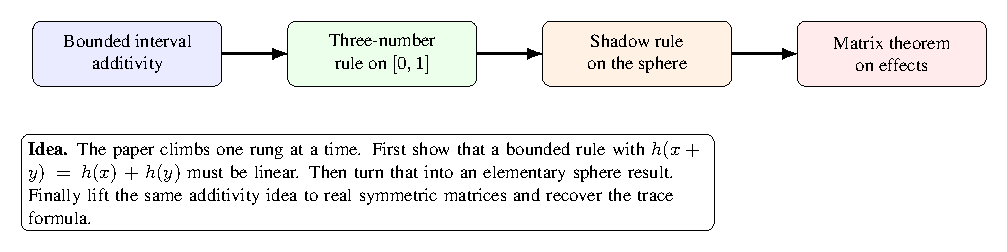
\includegraphics[width=0.98\linewidth]{../figure_assets/proof_staircase/proof_staircase.pdf}
\caption{The proof route used in the paper. Each step keeps the ideas concrete and postpones the matrix theorem until the one-variable and sphere warmups are already in place.}
\label{fig:staircase}
\end{figure}

\begin{figure}[t]
\centering
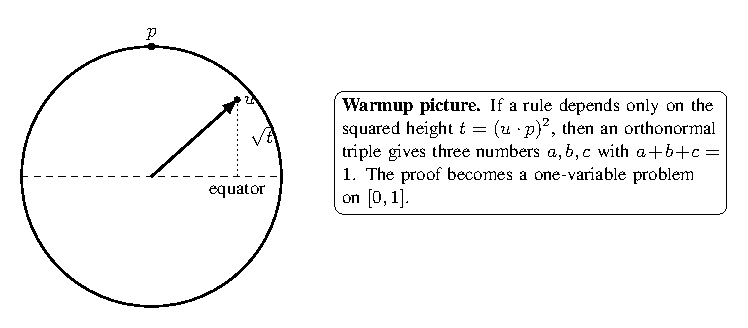
\includegraphics[width=0.98\linewidth]{../figure_assets/sphere_shadow/sphere_shadow.pdf}
\caption{The high-school warmup picture. A rule that depends only on squared height turns an orthonormal triple on the sphere into a three-number identity on $[0,1]$.}
\label{fig:shadow}
\end{figure}


The main paper theorem will come from the same idea twice: bounded additivity forces linearity. We start in one variable because that version is simple enough to explain to a strong high-school student.

\begin{lemma}[Bounded interval additivity]
Let $h:[0,1]\to\mathbb{R}$ be bounded. Suppose that
\[
h(x+y)=h(x)+h(y)
\]
whenever $x,y \ge 0$ and $x+y \le 1$. Then $h(t)=ct$ for some constant $c$ and all $t\in[0,1]$.
\end{lemma}

\begin{proof}
First, $h(0)=0$ because $h(0)=h(0+0)=h(0)+h(0)$.

For every positive integer $n$,
\[
h(1)=h\Bigl(\underbrace{\tfrac1n+\cdots+\tfrac1n}_{n \text{ times}}\Bigr)=n\,h(1/n),
\]
so $h(1/n)=h(1)/n$. Therefore, for every rational number $m/n \in [0,1]$,
\[
h(m/n)=m\,h(1/n)=(m/n)\,h(1).
\]

Now use boundedness. Let $|h(t)|\le M$ on $[0,1]$. If $0<u\le 1/n$, then
\[
n|h(u)|=|h(nu)|\le M,
\]
so $|h(u)|\le M/n$. Thus $h(u)\to 0$ as $u\to 0^+$.

Take any real $x\in[0,1]$ and choose rationals $q_k\to x$. Then
\[
h(x)-h(q_k)=h(x-q_k)
\]
when $q_k\le x$, and the right-hand side tends to $0$. Since $h(q_k)=q_k h(1)$ for rational $q_k$, it follows that
\[
h(x)=x\,h(1).
\]
So $h(t)=ct$ with $c=h(1)$.
\end{proof}

\begin{theorem}[Three-number rule]
Let $g:[0,1]\to\mathbb{R}$ be bounded. Suppose that
\[
g(a)+g(b)+g(c)=1
\]
whenever $a,b,c\in[0,1]$ and $a+b+c=1$. Then $g$ is affine:
\[
g(t)=\beta+\alpha t
\]
for constants $\alpha,\beta$ satisfying $\alpha+3\beta=1$.
\end{theorem}

\begin{proof}
Let $\beta=g(0)$ and define $h(t)=g(t)-\beta$. Compare the two valid triples
\[
(x,y,1-x-y)
\quad\text{and}\quad
(x+y,0,1-x-y).
\]
Subtracting the corresponding identities gives
\[
h(x+y)=h(x)+h(y)
\]
whenever $x+y\le 1$. Since $h$ is bounded, the lemma implies $h(t)=\alpha t$ for some $\alpha$. Hence $g(t)=\beta+\alpha t$.

Finally, plugging $(1,0,0)$ into the hypothesis gives
\[
g(1)+2g(0)=1,
\]
which is exactly $\alpha+3\beta=1$.
\end{proof}

\begin{corollary}[Squared-height sphere rule]
Fix a unit vector $p\in\mathbb{R}^3$. Suppose $F$ assigns a real number to each unit vector $u\in S^2$ and depends only on the squared height relative to $p$:
\[
F(u)=g((u\cdot p)^2).
\]
If
\[
F(u)+F(v)+F(w)=1
\]
for every orthonormal triple $(u,v,w)$ in $\mathbb{R}^3$, then
\[
F(u)=\beta+\alpha (u\cdot p)^2
\]
with $\alpha+3\beta=1$.
\end{corollary}

\begin{proof}
For every orthonormal triple $(u,v,w)$,
\[
(u\cdot p)^2+(v\cdot p)^2+(w\cdot p)^2=\|p\|^2=1,
\]
because $(u,v,w)$ is an orthonormal basis of $\mathbb{R}^3$. So the three numbers
\[
a=(u\cdot p)^2,\quad b=(v\cdot p)^2,\quad c=(w\cdot p)^2
\]
always satisfy $a+b+c=1$. The theorem applies directly to $g$.
\end{proof}

The sphere corollary is not the full Gleason problem. It is a warmup. But it already captures the central pattern: a rule constrained on orthogonal triples becomes rigid because the underlying additivity is bounded.
